\documentclass[twocolumn,10pt]{asme2e}
\usepackage{graphicx}
\usepackage{hologo}
\usepackage{amsmath}
\usepackage{caption}
\usepackage{verbatim} % for comments
\usepackage[table,xcdraw]{xcolor}
\usepackage[utf8]{inputenc}
\usepackage{hyperref}
\special{papersize=8.5in,11in}

\conffullname{the ASME 2025 \vspace{1 mm}\\ International Design Engineering Technical Conferences \vspace{1 mm}\&\\ Computers and Information in Engineering Conference\vspace{1 mm}}
\confshortname{\vspace{1 mm}IDETC/CIE2025\vspace{1 mm}}
\vspace{1 mm}
\confdate{August 17-20}
\confyear{2025}
\confcity{Anahiem, California}
\confcountry{USA}
\papernum{DETC2025-XXXXX}

\title{ \vspace{-10 mm} A Multidisciplinary Design Optimization Framework for Wave-Driven Desalination Systems}
%%% first author
\author{Nate DeGoede$^1$\thanks{Corresponding Author}, Maha Haji$^1$
    \affiliation{
	$^1$Sibley School of Mechanical and Aerospace Engineering\\
	Cornell University\\
	Ithaca, New York 14853\\
    Email: \{njd76, maha\}@cornell.edu 
    }
}

\begin{document}
\maketitle
% decrease the space buffer around equations
\setlength{\abovedisplayskip}{10pt}
\setlength{\belowdisplayskip}{10pt}

\begin{abstract}

This paper
\end{abstract}


\section{Introduction}

The world is facing a water crisis. Fresh water demand is expected to grow over 40\% by 2050 \cite{watershortage2015}. This increase in demand coupled with other factors like droughts, urbanization, and uneven distribution of water resources will result in significant stress on water resources. Desalination through processes like SeaWater Reverse Osmosis (SWRO) is one way to alleviate stress on these essential freshwater resources. However, these processes require a large amount of energy, which if provided through fossil fuels would exacerbate the climate crisis, further stressing freshwater resources \cite{nytdrought}. Therefore, it is essential for sustainable energy sources to be used to power SWRO. 

Wave Energy Converters (WECs) have not seen the same level of development as other renewable energy sources like wind and solar. However, SWRO provides a unique opportunity for WECs to develop \cite{blue_econ}. Desalination, a Blue Economy application, needs to take place near the coast, so co-location with marine energy is guaranteed. Additionally, WECs have an advantage over their solar competitors in suitability of power for SWRO. The primary energy demand of SWRO is in the pressurization of seawater, and WECs can provide this directly through a hydraulic style Power Take-Off (PTO) system in the form of a Wave-Driven Desalination System (WDDS) \cite{Davies2005}. The direct nature of this power transfer has the opportunity to reach efficiencies not possible with other renewable energy sources requiring an intermediate step to convert the energy to electricity. 

Multidisciplinary Design Optimization (MDO) strategies like Control Co-Design (CCD) have been applied to electricity generating WECs with great success \cite{Stroefer2023,PenaSanchez2022,Rosati2023,Grasberger2024}. Michelén Ströfer et al. used CCD with PTO design to get a 22\% increase in electrical power output. Additionally, all these studies have shown that a wholistic model of a WEC system is essential to predict behavior. The coupled dynamics between the waves, WEC, PTO, and controls are essential to understand the system's behavior. Although these studies have showed the importance of MDO approaches and wholistic models for electricity generating WECs, these approaches have not been applied to WDDS.

This study looks to fill this gap and apply a wholistic MDO framework to WDDS. This framework is then used in a design of experiments as a precursor to an MDO study for the optimization of freshwater production. For this study, a simple WDDS architecture is presented, and shown in Fig \ref{fig:WDDS}. This architecture uses an Oscillating Surge Wave Energy Converter (OSWEC) to drive a piston pump witch takes in seawater and sends it back to shore where a SWRO plant is located. The SWRO plant then uses the high pressure seawater provided by the OSWEC to produce freshwater. This type of system is similar to systems that have been studied in the past \cite{Yu2018,Suchithra2022,Mi2023,Simmons2024}, but without the energy recovery unit that many of these studies have. The energy recovery unit is proven to increase the performance, but is removed from this study to simplify the system and focus on the MDO aspects of the study. 

\begin{center}
    \includegraphics[width=\linewidth]{../figs/WDDS.png}
    \captionof{figure}{Simple Wave-Driven Desalination System (WDDS) Concept Sketch.}
    \label{fig:WDDS}
\end{center}

It is worth noting that the concept sketch shown in Fig \ref{fig:WDDS} does not show some hydraulic elements included in this study, such as the hydraulic accumulator, pressure relief valve, brine side throttle valve, and various directional valves. These hydraulic elements are shown in the hydraulic circuit diagram, Fig \ref{fig:hydraulics}.

\begin{center}
    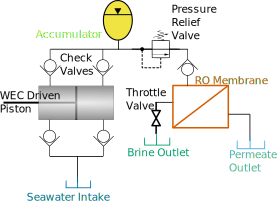
\includegraphics[width=\linewidth]{../figs/hydraulic_circuit.pdf}
    \captionof{figure}{Simple Wave-Driven Desalination System (WDDS) Concept Sketch.}
    \label{fig:hydraulics}
\end{center}

In the following sections...

All code for this study can be accessed at \href{https://github.com/symbiotic-engineering/mdo_wd2}{https://github.com/symbiotic-engineering/mdo\_wd2}.

\section{Problem Formulation}
\subsection{Multidisciplinary Design Optimization Framework}
\subsection{Design Space}

\section{System Modeling}
\subsection{Hydrodynamics}

The Cummins equation is commonly used to calculate the motion of a wave energy converter and is shown below.
\begin{equation}
    \label{eq:cummins}
    I\ddot{\Xi} = f_e - f_r - f_d - f_{hs} - f_{pto}  
\end{equation}
where $I$ is the inertia matrix, a function of WEC mass (a design variable), $\Xi$ is the body motion vector, $f_e$ is the excitation force, $f_r$ is the radiation force, $f_d$ is the drag force, $f_{hs}$ is the hydrostatic force, and $f_{pto}$ is the PTO force. The PTO force is entirely modeled in the system dynamics module, and the drag force is removed to assume linear potential flow. The hydrostatic force accounts for the buoyancy of the WEC and a tendency to return to an equilibrium position, it is assumed to follow the form below.
\begin{equation}
    \label{eq:hydrostatic}
    f_{hs} = K_{hs} \Xi
\end{equation}
where $K_{hs}$ is the hydrostatic stiffness matrix. The radiation force is accounts for the radiated waves generated by the WEC motion and is assumed to follow the form below.
\begin{equation}
    \label{eq:radiation}
    f_r = A \ddot{\Xi} + B \dot{\Xi}
\end{equation}
where $A$ and $B$ are the added mass and radiation damping matrices respectively. This leaves us with 4 terms required to fully characterize the hydrodynamics of the WEC: the excitation force, the inertia matrix, the added mass matrix, and the radiation damping matrix. To calculate these, we utilize the open source Boundary Element Method (BEM) solver Capytaine \cite{ancellin_capytaine_2019}. 

%Wave-structure interactions are commonly characterized using linear potential flow theory. The theory assumes the fluid velocity field $\vec{v}$ is the gradient of some complex potential ($\phi$), where $\vec{v}=\nabla \phi$ and $\phi$ satisfies the Laplace equation, $\nabla^2 \phi = 0$. It also assumes inviscid, irrotational, and incompressible flow. $\phi(x,y,z)$ is complex velocity potential represented in $ \Phi = \mathbb{Re}(\phi e^{-j\omega t})$. The boundary conditions for the associated boundary value problem (BVP) are at the sea bed, immersed surface of the body and far field radiation condition \citep{Falnes_2002}. 

%Similarly, the hydrodynamics module also calculates the hydrostatic stiffness matrix of the WECs ($C_{33}$). For a stably floating body $b$ a hydrodynamic analysis is then performed $(M_{bb} = \rho g V_b)$ .  The density of sea water is $\rho$, $g$ is acceleration due to gravity, $V_b$ is the submerged volume of the WEC, and $M_{bb}$ is the mass of the WEC.

%Most common solvers modeling hydrodynamics are based on a reformulation of the governing PDE (Laplace equation) and associated boundary conditions as boundary integral equations (BIEs). These BIEs and the associated boundary element method (BEM) are well-suited for wave problems in unbounded domains, complex geometries and arbitrary arrangement of bodies \citep{bem_wave}.  In this method, only the body geometry is discretized into a mesh with panels and Green's identity is used to derive a boundary integral equation which is then discretized into a linear system. Thus, this method is ideal for design (size and shape) optimizations as only the body surface needs to be meshed. This is advantageous compared to meshing the domain (large ocean) around the floating body. This method is implemented in the open-source frequency-domain BEM code Capytaine, our solver of choice \citep{ancellin_capytaine_2019} \citep{babarit_theoretical_2015}. 

\subsection{Seawater Desalination Parameters}
From the capacity variable along with parameters defining the composition of the seawater, the desalination module calculates several parameters necessary for the calculation of the full description of the SWRO plant. The governing equation for the reverse osmosis process we use is shown below.
\begin{equation}
    \label{eq:ro}
    Q_p = A_w A (\Delta P - \Delta \pi)
\end{equation}
where $Q_p$ is the permeate flow rate, $A_w$ is the water permeability coefficient, $A$ is the membrane area, $\Delta P$ is the pressure difference across the membrane, and $\Delta \pi$ is the osmotic pressure difference across the membrane. The osmotic pressure is calculated using the van't Hoff equation shown below.
\begin{equation}
    \label{eq:osmotic_pressure}
    \pi = iCRT
\end{equation}
where $i$ is the number of ions produced per molecule of solute, $C$ is the concentration of the solute, $R$ is the ideal gas constant, and $T$ is the temperature. An alternative way to calculate the osmotic pressure difference specific to seawater is to use the formula presented by Applegate \cite{separationprocesses}.
\begin{equation}
    \label{eq:osmotic_pressure_applegate}
    \pi = 1.12 T \sum m_i
\end{equation}
where $\sum m_i$ is the summation of the molarities of dissolved ions in seawater. In this study we will be focusing on the equation presented in eq \ref{eq:osmotic_pressure}, but equation \ref{eq:osmotic_pressure_applegate} is included for reference as a potential alternative for applications where there is a stronger understanding of the composition of the seawater at a specific site. 

In this study, we set $\Delta \pi$ to the osmotic pressure of the seawater (assuming an osmotic pressure of the permeate side of 0).

For the water permeability coefficient $A_w$ we use the constant value ($2.57\times10^{-12}$ m$^3$/N-s) used by Yu and Jenne \cite{Yu2018}. We use the same RO membrane, the SW30HR-380 Dry from DuPont \cite{SW30HR380}, justifying our use of their coefficient. The membrane area $A$ is then calculated as the quotient of the capacity of the system (a design variable) divided by the designed flux of the RO membrane. The flux of the membrane is calculated as the quotient of the flow rate and the membrane area, both found off the datasheet \cite{SW30HR380}.

At this point the governing equation \ref{eq:ro} is only a relationship between pressure and flow rate. For the system dynamics we would like this to be defined as an resistance style relationship. The resistance of the membrane ($R_m$) is simply $frac{1}{A_w A}$, and is used in the system dynamics module.

To avoid running the system above capacity, a pressure relief valve is included and set to the pressure indicated in the following equation.
\begin{equation}
    P_{\text{relief}} = \text{capacity}R_m + \Delta \pi
    \label{eq:pressure_relief}
\end{equation}
this ensures that if the flow exceeds the capacity of the system, the pressure relief valve will open. It is worth noting here that since the membrane resistance, $R_m$, contains $\text{capacity}^{-1}$, the pressure relief setting does not change given the current design space and model for membrane resistance. It remains a dependant variable though to enable flexibility for the system to adapt to an alternative design space or model.

For any flow to go through the membrane, a resistance on the brine side is necessary. This resistance can be thought of as a throttle valve, or could be an energy recovery unit in a more complex system. In this study we use a simple throttle valve model, with a constant resistance $R_t$. This resistance is calculated such that when the system runs at full capacity, it also runs at the recommended recovery ratio given the SW30HR-380 membrane and the specified seawater composition.
\begin{equation}
    R_t = \frac{P_{\text{relief}}}{\text{capacity}(\frac{1}{\text{recovery ratio}} - 1)}
\end{equation}

\subsection{System Dynamics}

To take advantage of MathWorks specific tools, the WDDS system dynamics are modeled in MATLAB+Simulink. The system dynamics captures the interactions between the WEC and PTO. The model for each of these components is explained in more detail below. 

\subsubsection{Wave Energy Converter}

Using the hydro coefficients found in the hydro module, the WEC dynamics are modeled using WEC-Sim \cite{wecsim}. WEC-Sim is an open source software developed by NREL and Sandia that models WEC system dynamics using hydro coefficients in a Simulink system model. WEC-Sim holds advantages over other WEC simulating software tools because by simulating in the time domain it can capture complexity and non-linearities that others can only approximate. The WEC is modeled as a two body system, with the base fixed to the seafloor and the flap limited to a one degree of freedom (pitch). The WEC model also includes the mechanism to drive the piston. With the intake location, hinge location, and PTO joint location all defined according to Fig. \ref{fig:mechanism}. The block diagram used to model the WEC is shown in Fig. \ref{fig:wec_simscape}.
\begin{center}
    \includegraphics[width=\linewidth]{../figs/wecsimscape.pdf}
    \captionof{figure}{Model of the WEC in Simscape.}
    \label{fig:wec_simscape}
\end{center}

\subsubsection{Power Take-Off}

The desalination hydraulic circuit shown in Fig \ref{fig:hydraulics} is modeled using the isothermal liquid domain from the Simscape fluids toolbox. This domain is specialized for modeling hydraulic systems, and is a good fit for modeling the dynamics of the hydraulic circuit presented. The high level Simscape PTO model is shown in Fig. \ref{fig:hydraulic_simscape}.

\begin{figure*}[t]  % The [t] option places the figure at the top of the page
    \centering
    \includegraphics[width=\linewidth]{../figs/hydraulic_simscape.pdf}
    \captionof{figure}{Model of the hydraulic circuit in Simscape.}
    \label{fig:hydraulic_simscape}
\end{figure*}

From this high level view, we can see the main components of the hydraulic circuit. The ``piston\_cylinder" block contains the piston and directional valves, then we have the accumulator and pressure relief valve, next the reverse osmosis membrane is modeled in the ``simple\_ro" block, and then finally the throttle valve on the brine side.

The ``piston\_cylinder" subsystem is further broken down in Fig. \ref{fig:piston_simscape}. In this model we present a single piston double acting piston, however the dynamics would not change much if the piston area variable was split into multiple pistons instead of a single large piston. Another feature of note is the use of three way controlled directional valves instead of check valves. This is to make things easier on the solver, while not changing the dynamics of the system.

\begin{center}
    \includegraphics[width=\linewidth]{../figs/pistonsimscape.pdf}
    \captionof{figure}{Model of the piston and directional valves in Simscape.}
    \label{fig:piston_simscape}
\end{center}

The ``simple\_ro" subsystem is broken down in Fig. \ref{fig:ro_simscape}. This subsystem includes a check valve to prevent forward osmosis in low energy sea states, and then the membrane resistance and osmotic pressure blocks allow for a simscape representation of the reverse osmosis equation presented in eq \ref{eq:ro}. The membrane resistance block is a linear resistance on the volumetric flow rate, and the osmotic pressure block applies a pressure on the permeate side equal to the osmotic pressure difference as calculated in equations \ref{eq:osmotic_pressure} or \ref{eq:osmotic_pressure_applegate}.

\begin{center}
    \includegraphics[width=\linewidth]{../figs/desalsimscape.pdf}
    \captionof{figure}{Model of the reverse osmosis membrane in Simscape.}
    \label{fig:ro_simscape}
\end{center}

\subsubsection{Coupled Solver}

The two subsystems of the WEC and PTO are then coupled through as shown in Fig. \ref{fig:coupled_system}. Where the velocity and acceleration signals are fed as inputs to the PTO from the WEC, and the force is fed back from the PTO to the WEC. WEC-Sim uses this coupled system to simulate the system dynamics of the WDDS. The solver used is MATLAB's ode4 solver, a fourth order Runge-Kutta solver, and is used with a 0.1s time step. 

\begin{center}
    \includegraphics[width=\linewidth]{../figs/coupledsimscape.pdf}
    \captionof{figure}{Model of the coupled WEC and PTO in Simscape.}
    \label{fig:coupled_system}
\end{center}

\subsection{Economics}

Our objective function LCOW is calculated using the AWP from the system dynamics module and the costs calculated from this economic module. We use a simple cost model with costs split into two categories: capital costs (CAPEX) and operational (OPEX). The equation below for LCOW is a modification of the LCOE equation proposed by the U.S. Department of Energy \cite{LCOE_DOE}
\begin{equation}
    \text{LCOW} = \frac{(\text{FCR}\times\text{CAPEX}) + \text{OPEX}}{\text{AWP}}
\end{equation}
where FCR is the fixed charge rate, 10.8\% based on te assumptions made in the U.S. Department of Energy report \cite{LCOE_DOE}. The CAPEX and OPEX are split into three sections based on the three main sections of design variables: the WEC, the PTO, and the desalination plant. It is worth noting that this cost model is not intended to be a perfect representation of the total system costs, but rather a way to quantify estimated savings between different designs as a way to demonstrate the impact of an MDO approach to this problem. An explanation of the cost model for each section is given below.

\subsubsection{Wave Energy Converter}

Cost models for WECs come with a lot of uncertainty. With limited real world data, there is a substantial limitation on how accurate a cost model can be. This presents significant challenged for studies like this where a levelized cost is used as an objective. Despite the challenge in creating an accurate cost model, it is still possible to build a useful cost model that while not perfect, can capture trends necessary for the comparison of different designs. Grasberger et al. use a simple cost model for their OSWEC CCD study \cite{Grasberger2024}. Their cost model is a function of the surface area of the float with one term scaled linearly and the other logarithmically. The linear term captures cost associated with the structural components (the flap, base, and mooring), while the logarithmic term captures other expenses (PTO, monitoring, other OPEX) which are less dependent on the size of the float. These two cost terms are shown in the equation below
\begin{equation}
    \text{Cost} = C_{1,ref}(A_{x}/A_{ref}) + C_{2,ref}(1 + \text{log}(A_{x}/A_{ref}))
\end{equation}
where $A_{x}$ is the surface area of the float, $A_{ref}$ is the surface area of the reference float, and $C_{1,ref}$ and $C_{2,ref}$ are the costs of the reference float associated with the two terms. Due to the equation's dependence on the surface area and costs of a reference WEC, it is important to have an accurate cost model for a reference WEC. Luckily, while general WEC cost equations are hard to find, the reference model studies from NREL provide some thoroughly documented cost estimates \cite{rm5}. The RM5 reference model is an OSWEC, like the one used in this study, and therefore will be the reference point used in this study. It is worth noting that due to the replacement of the electricity generating PTO with the SWRO PTO, the PTO costs are not included in this study. Additionally, many of the mooring costs are not considered because this system is a nearshore fixed-bottom WEC, and many installation and other overhead design costs are not included as they likely will not scale with the size of the WEC.

\subsubsection{Power Take-Off}

\subsubsection{Desalination Plant}
The costs associated with the desalination plant are split into two categories: capital costs and operational costs. The capital costs are the costs associated with the construction of the plant, while the operational costs are the costs associated with the yearly operation of the plant. Cost models for SWRO desalination plants of this scale (thousands of m$^3$/day) are quite rare, and generally either quite poorly documented or implemented. The majority of well documented economic studies are for much larger plants (hundreds of thousands of m$^3$/day) \cite{Slocum2016,Haefner2023,roopexcurve,Wittholz2008}. Studies that focus on the economic modeling of smaller plants generally have poorly documented cost estimates for how to estimate SWRO plant costs \cite{Elkadeem2024,Goekcek2016}. Another study, specific to wave driven desalination using the Desalination Economic Evaluation Program (DEEP 5.1) developed by the International Atomic Energy Agency for a unit CAPEX cost \cite{Yu2022}. However, the DEEP 5.1 model itself is poorly documented \cite{DEEP5manual}, making it hard to know if this number is a good representation. 

This study instead uses a a cost model based on the cost estimation methodology presented by Voutckov in his book "Desalination Project Cost Estimating and Management" \cite{voutch}. Using the cost curves from sections 4 (CAPEX) and 5 (OPEX), a cost model that can be customized to the specific needs of a given project can be created. Each curve was fitted to simple power fit shown in the equation below
\begin{equation}
    y = a \cdot x^b
\end{equation}
This form was chosen because it ensures there won't be strange behaviors as the low end of the range. Other forms such as polynomial fits could result in negative costs at the low end of the range, which is nonsensical.

\bibliographystyle{ieeetr}
\bibliography{biblio}
\end{document}